



\subsubsection{Meteor yleisesti}
% sitatatti order kussee.. tässä sitatoidaan meteor b sitatoidaan ekaks ja tässä sitatoidaan mongo i kun senkin pitäisi olla mongo a
% eli kaikki pitää siirtää vähän
% nämä muutokset pitäisi tehdä kun kaikki sitaatit on lisätty missing sitateista

%iso morphic src jos ei käy niin käytä tätä
%https://web.archive.org/web/20221206181248/https://old.gigaom.com/2014/12/27/meteor-wants-to-be-the-warp-drive-for-building-real-time-apps/
% Jonathan Vanian

%



Meteor on full-stack JavaScript web-framework ja on itsessään avoimeen lähdekkoodiin perustuva \labciteend{meteor24b}{}
% poislukien on vähän scuffed imo
Poislukien meteorin mukaan paketoimaa mongodb tietokantaa, joka toimii Server Side Public Lisenssillä.\labciteend{mongodb24i}
Meteor on suunniteltu nopeaan kehittämiseen monelle laitteille ja nopeaan käyttöönottoon ja se mahdollistaa isomorphiseen koodin kirjoittamisen, 
eli koodiin joka on samanlaista palvelimella kuten clientillä.\labcite{Kuster23} % en tiedä onko hyvä src mutta on totta joten pitäis löytää jokue
Meteor ei määritä käytettyä front-end teknologiaa vaan sillä on integraatio moneen yleiseen frontend-framework:kiin, kuten Vue, React, Svelte tai Angular \labciteend{meteor24a}{}
Tämä antaa lisä joustoa Meteorille sillä se antaa mahdollisuuden monelle sovelluskehittäjälle joilla ei ole kokemusta tietystä front-end teknologiasta.
\medskip

% asio ok mut kirjota paremmin ja uusiks varm gpt on ok täs vaihees
% asia ei ole ok tässä pitää selittää enemmän isomorphisesta jos selitäteään mitään. tosin voi poistaa jos halutaan
% paremmin alku. plus se että se on fullstack ei tarkoita sitä että sen mukana aina tulee palvelin. meteor päätti laittaa palvelimen samalla käynnistymää. plus se että se on fullstack ei tarkoita sitä että sen mukana aina tulee palvelin. meteor päätti laittaa palvelimen samalla käynnistymään
Meteor on fullstack, joten kun sen käynnistää se käynnistää samalla palvelimen ja clientin.
Tiedostorakenteessa on erityks kansioita kuten server ja client jota käyttäen Meteor tietää mitä koodia pitää ladata clientille ja mitä palvelimelle.
%more text
\medskip



    
% https://www.meteor.com/
% viitattu 28.5

% tukee sana pitää vaihtaa sillä me käytetään sitä itemeissä
Lisäksi Meteor tukee monta ominaisuutta \labcite{meteor24a}:
\begin{itemize}
    \item Tukee monta Front-end kirjastoa ja frameworkkkia
    \item Tukee Typescriptiä
    \item Sisään rakennettu käyttäjä systeemi
    \item Toimii monella laitteella
    \item Helppo ja nopea käyttöönottaa 
\end{itemize}
\medskip


Meteor paketoi mukaansa käyttäjä paketin jota käyttäen kehitäjä voi nopeasti luoda authentikaatio järjestelmän.
Käyttäjä paketti antaa helpon integraation muiden kirjautumis palvelujen kanssa kuten facebook, github, google ym.
Käyttäjä paketti on myös integroitu muihin Meteorin ominaisuuksiin kuten metodeihin. \labcite{meteor24c}
%maby more txt



\subsubsection{Meteor metodit}

%ensimmäinen kappale pitää kirjoittaa uusiks. siinä ei ole tarpeeksi tekstiä eikä siinä selitetä kaikkea mitä siinä pitää selittää

% https://www.ibm.com/docs/en/aix/7.2?topic=call-rpc-model
% 2.7 
% tätä voi sitatoida rpc hommissa

% toinen kappale
% metodi tekee koodista yksinkertaisemman. metodi tekee rajapinnasta helpomman lukea sillä

% mahdollinen kappale rike kolmannessa kappaleessa


Meteor käyttää Etäkäsittelykutsu (eng Remote procedure call) rajapintaa perinteisen RESTful rajapinnan sijasta \labciteend{meteor24a}
Etäkäsittelykutsussa mallissa asiakasohjelma lähettää palvelinohjelmalle kutsuviestin.
Palvelinohjelma käsittelee kutsuviestin ja suorittaa halutun toiminnon ja palauttaa vastaviestin asiakasohjelmalle.\labcite{ibm23}
Meteorin metodit ominaisuus toimii Etäkäsittelykutsu rajapintana clientin ja palvelimen välillä. 
Tämä antaa clientin mahdollisuuden kutsua palvelimelta funktioita Meteorin kautta.
\medskip


% metodit tekee koodista yksinkertaisempaa

Metodit määritetään ja suoritetaan palvelimella kuten kuvassa \nextImageCount.
%selitä yksinkertaisemman eri tavalla
Metodit tekee myös koodista yksinkertaisemman sillä clientin ei tarvitse tehdä GET tai POST requesteja palvelimelle, kun halutaan palvelimen tehdä jotain. 
Ja koska metodi kutsu on myös isomorphinen, metodeja on helppo uudelleen käyttää palvelimella.
Metodi funktio käyttää JavaScriptin "this"{} ominaisuutta. 
Sitä käyttäen metodiin voidaan antaa kontekstia kutsujasta.
Tässä kontekstissa voi nähdä esimerkiksi onko kutsuja kirjautunut sisään, tai onko kutsujalla oikeat oikeudet kutsua metodia, 
helpottaen turvallisuuden lisäämista rajapintaan.
\bigskip

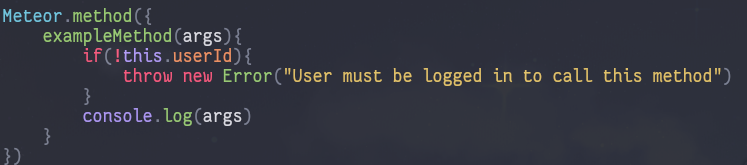
\includegraphics[width=15cm]{src/public/methodexample.png}\\
Kuva \getImgCount {}. Meteor metodin määritelmä
\medskip

% onko tässä passiivi rike jossain
Kuvassa on meteor metodin määritelmä. "exampleMethod"{} metodi katsoo, onko "this"{} ominaisuudessa käyttäjä tunnusta, näin voimme tietää onko kutsuja kirjautunut sisään,
jos käyttäjä ei ole kirjautunut sisään heitetään error viesti, joka välitetään kutsujalle.
Jos käyttäjä on kirjautunut sisään tulostetaan argumentit. 
\medskip




\subsubsection{Meteor ecosysteemi}


% eka kappale pitää vain kirjoittaa vähän paremmin muuten ok
%
%build system pitää vissii vähä paremmin selittää...
% sdelitetäänkö build system vai.... vaihdetaanko sana johonkin toiseen vaa


% yhdistä lauseet paremmin, elä aloita jokainen lause Meteor sanalla
Meteor ylläpitää omaa paketointi ecosysteemiään, nämä
paketit ovat isomorphisia, eli ne toimivat palvelimella ja clientillä \labciteend{pranav17}{}
Meteorilla on ensimmäisen osapuolen paketteja, joita itse meteor tiimi ylläpitää ja kolmannen osapuolen paketteja,
joita yhteisö ylläpitää. Nämä kolmannen osapuolen paketit voi ladata Meteorin paketti palvelimelle Athmosphere:lle. \labcite{sanders15}
\medskip


Athmosphere on Meteorin ylläpitämä paketti palvelin, johon käyttäjät voivat ladata paketteja tai kirjastoja, jotka ovat suunnattu toimimaan meteorin kanssa.
NPM paketit (eng Node package manager) ovat suunnattu toimimaan Node ympäristössä, ja vaikka ratkaisuja on käyttää NPM paketteja selaimella, 
%build system
Athmosphere paketit voi hyötykäyttää Meteorin build systeemiä, jonka avulla paketin kehittäjä voi määritellä mitkä osat ladataan selain puolelle ja mitkä palvelimelle.\labcite{meteor24d}

